% Options for packages loaded elsewhere
\PassOptionsToPackage{unicode}{hyperref}
\PassOptionsToPackage{hyphens}{url}
%
\documentclass[12pt]{article}
\usepackage{geometry}
\geometry{left=3.18cm, right=3.18cm, top=2.54cm, bottom=2.54cm}
\usepackage{amsmath,amssymb}
\usepackage{lmodern}
\usepackage{iftex}
\ifPDFTeX
  \usepackage[T1]{fontenc}
  \usepackage[utf8]{inputenc}
  \usepackage{textcomp} % provide euro and other symbols
\else % if luatex or xetex
  \usepackage{unicode-math}
  \defaultfontfeatures{Scale=MatchLowercase}
  \defaultfontfeatures[\rmfamily]{Ligatures=TeX,Scale=1}
\fi
% Use upquote if available, for straight quotes in verbatim environments
\IfFileExists{upquote.sty}{\usepackage{upquote}}{}
\IfFileExists{microtype.sty}{% use microtype if available
  \usepackage[]{microtype}
  \UseMicrotypeSet[protrusion]{basicmath} % disable protrusion for tt fonts
}{}
\makeatletter
\@ifundefined{KOMAClassName}{% if non-KOMA class
  \IfFileExists{parskip.sty}{%
    \usepackage{parskip}
  }{% else
    \setlength{\parindent}{0pt}
    \setlength{\parskip}{6pt plus 2pt minus 1pt}}
}{% if KOMA class
  \KOMAoptions{parskip=half}}
\makeatother
\usepackage{xcolor}
\IfFileExists{xurl.sty}{\usepackage{xurl}}{} % add URL line breaks if available
\IfFileExists{bookmark.sty}{\usepackage{bookmark}}{\usepackage{hyperref}}
\hypersetup{
  hidelinks,
  pdfcreator={LaTeX via pandoc}}
\urlstyle{same} % disable monospaced font for URLs
\usepackage{color}
\usepackage{fancyvrb}
\newcommand{\VerbBar}{|}
\newcommand{\VERB}{\Verb[commandchars=\\\{\}]}
\DefineVerbatimEnvironment{Highlighting}{Verbatim}{commandchars=\\\{\}}
% Add ',fontsize=\small' for more characters per line
\newenvironment{Shaded}{}{}
\newcommand{\AlertTok}[1]{\textcolor[rgb]{1.00,0.00,0.00}{\textbf{\footnotesize #1}}}
\newcommand{\AnnotationTok}[1]{\textcolor[rgb]{0.38,0.63,0.69}{\textbf{\textit{\footnotesize #1}}}}
\newcommand{\AttributeTok}[1]{\textcolor[rgb]{0.49,0.56,0.16}{\footnotesize #1}}
\newcommand{\BaseNTok}[1]{\textcolor[rgb]{0.25,0.63,0.44}{\footnotesize #1}}
\newcommand{\BuiltInTok}[1]{\footnotesize #1}
\newcommand{\CharTok}[1]{\textcolor[rgb]{0.25,0.44,0.63}{\footnotesize #1}}
\newcommand{\CommentTok}[1]{\textcolor[rgb]{0.38,0.63,0.69}{\textit{\footnotesize #1}}}
\newcommand{\CommentVarTok}[1]{\textcolor[rgb]{0.38,0.63,0.69}{\textbf{\textit{\footnotesize #1}}}}
\newcommand{\ConstantTok}[1]{\textcolor[rgb]{0.53,0.00,0.00}{\footnotesize #1}}
\newcommand{\ControlFlowTok}[1]{\textcolor[rgb]{0.00,0.44,0.13}{\textbf{\footnotesize #1}}}
\newcommand{\DataTypeTok}[1]{\textcolor[rgb]{0.56,0.13,0.00}{\footnotesize #1}}
\newcommand{\DecValTok}[1]{\textcolor[rgb]{0.25,0.63,0.44}{\footnotesize #1}}
\newcommand{\DocumentationTok}[1]{\textcolor[rgb]{0.73,0.13,0.13}{\textit{\footnotesize #1}}}
\newcommand{\ErrorTok}[1]{\textcolor[rgb]{1.00,0.00,0.00}{\textbf{\footnotesize #1}}}
\newcommand{\ExtensionTok}[1]{\footnotesize #1}
\newcommand{\FloatTok}[1]{\textcolor[rgb]{0.25,0.63,0.44}{\footnotesize #1}}
\newcommand{\FunctionTok}[1]{\textcolor[rgb]{0.02,0.16,0.49}{\footnotesize #1}}
\newcommand{\ImportTok}[1]{\footnotesize #1}
\newcommand{\InformationTok}[1]{\textcolor[rgb]{0.38,0.63,0.69}{\textbf{\textit{\footnotesize #1}}}}
\newcommand{\KeywordTok}[1]{\textcolor[rgb]{0.00,0.44,0.13}{\textbf{\footnotesize #1}}}
\newcommand{\NormalTok}[1]{\footnotesize #1}
\newcommand{\OperatorTok}[1]{\textcolor[rgb]{0.40,0.40,0.40}{\footnotesize #1}}
\newcommand{\OtherTok}[1]{\textcolor[rgb]{0.00,0.44,0.13}{\footnotesize #1}}
\newcommand{\PreprocessorTok}[1]{\textcolor[rgb]{0.74,0.48,0.00}{\footnotesize #1}}
\newcommand{\RegionMarkerTok}[1]{\footnotesize #1}
\newcommand{\SpecialCharTok}[1]{\textcolor[rgb]{0.25,0.44,0.63}{\footnotesize #1}}
\newcommand{\SpecialStringTok}[1]{\textcolor[rgb]{0.73,0.40,0.53}{\footnotesize #1}}
\newcommand{\StringTok}[1]{\textcolor[rgb]{0.25,0.44,0.63}{\footnotesize #1}}
\newcommand{\VariableTok}[1]{\textcolor[rgb]{0.10,0.09,0.49}{\footnotesize #1}}
\newcommand{\VerbatimStringTok}[1]{\textcolor[rgb]{0.25,0.44,0.63}{\footnotesize #1}}
\newcommand{\WarningTok}[1]{\textcolor[rgb]{0.38,0.63,0.69}{\textbf{\textit{\footnotesize #1}}}}
\usepackage{graphicx}
\makeatletter
\def\maxwidth{\ifdim\Gin@nat@width>\linewidth\linewidth\else\Gin@nat@width\fi}
\def\maxheight{\ifdim\Gin@nat@height>\textheight\textheight\else\Gin@nat@height\fi}
\makeatother
% Scale images if necessary, so that they will not overflow the page
% margins by default, and it is still possible to overwrite the defaults
% using explicit options in \includegraphics[width, height, ...]{}
\setkeys{Gin}{width=\maxwidth,height=\maxheight,keepaspectratio}
% Set default figure placement to htbp
\makeatletter
\def\fps@figure{htbp}
\makeatother
\setlength{\emergencystretch}{3em} % prevent overfull lines
\providecommand{\tightlist}{%
  \setlength{\itemsep}{0pt}\setlength{\parskip}{0pt}}
\setcounter{secnumdepth}{-\maxdimen} % remove section numbering
\ifLuaTeX
  \usepackage{selnolig}  % disable illegal ligatures
\fi
\usepackage{fontspec}
\setmainfont{Times New Roman}
\usepackage[font=small]{caption}
\usepackage[font=small]{subcaption}

\title{\bf A Mini Web Search Engine}
\author{Kevin Tan}
\date{}

\begin{document}

\maketitle

\textbf{\emph{Abstract---}Web search engines are irreplaceable in
people's daily lives. However, we tend to take them for granted and
ignore their principles. In this paper, a web search engine is built
from scratch, supporting indexing a large dataset into a compressed form
with limited memory, searching by multilingual conjunctive or
disjunctive queries, and interacting from a responsive web page or
command lines. By designing and implementing the search engine, the
author gains a deeper understanding of web search engines and acquires
practical skills for similar tasks.}

\begin{figure}
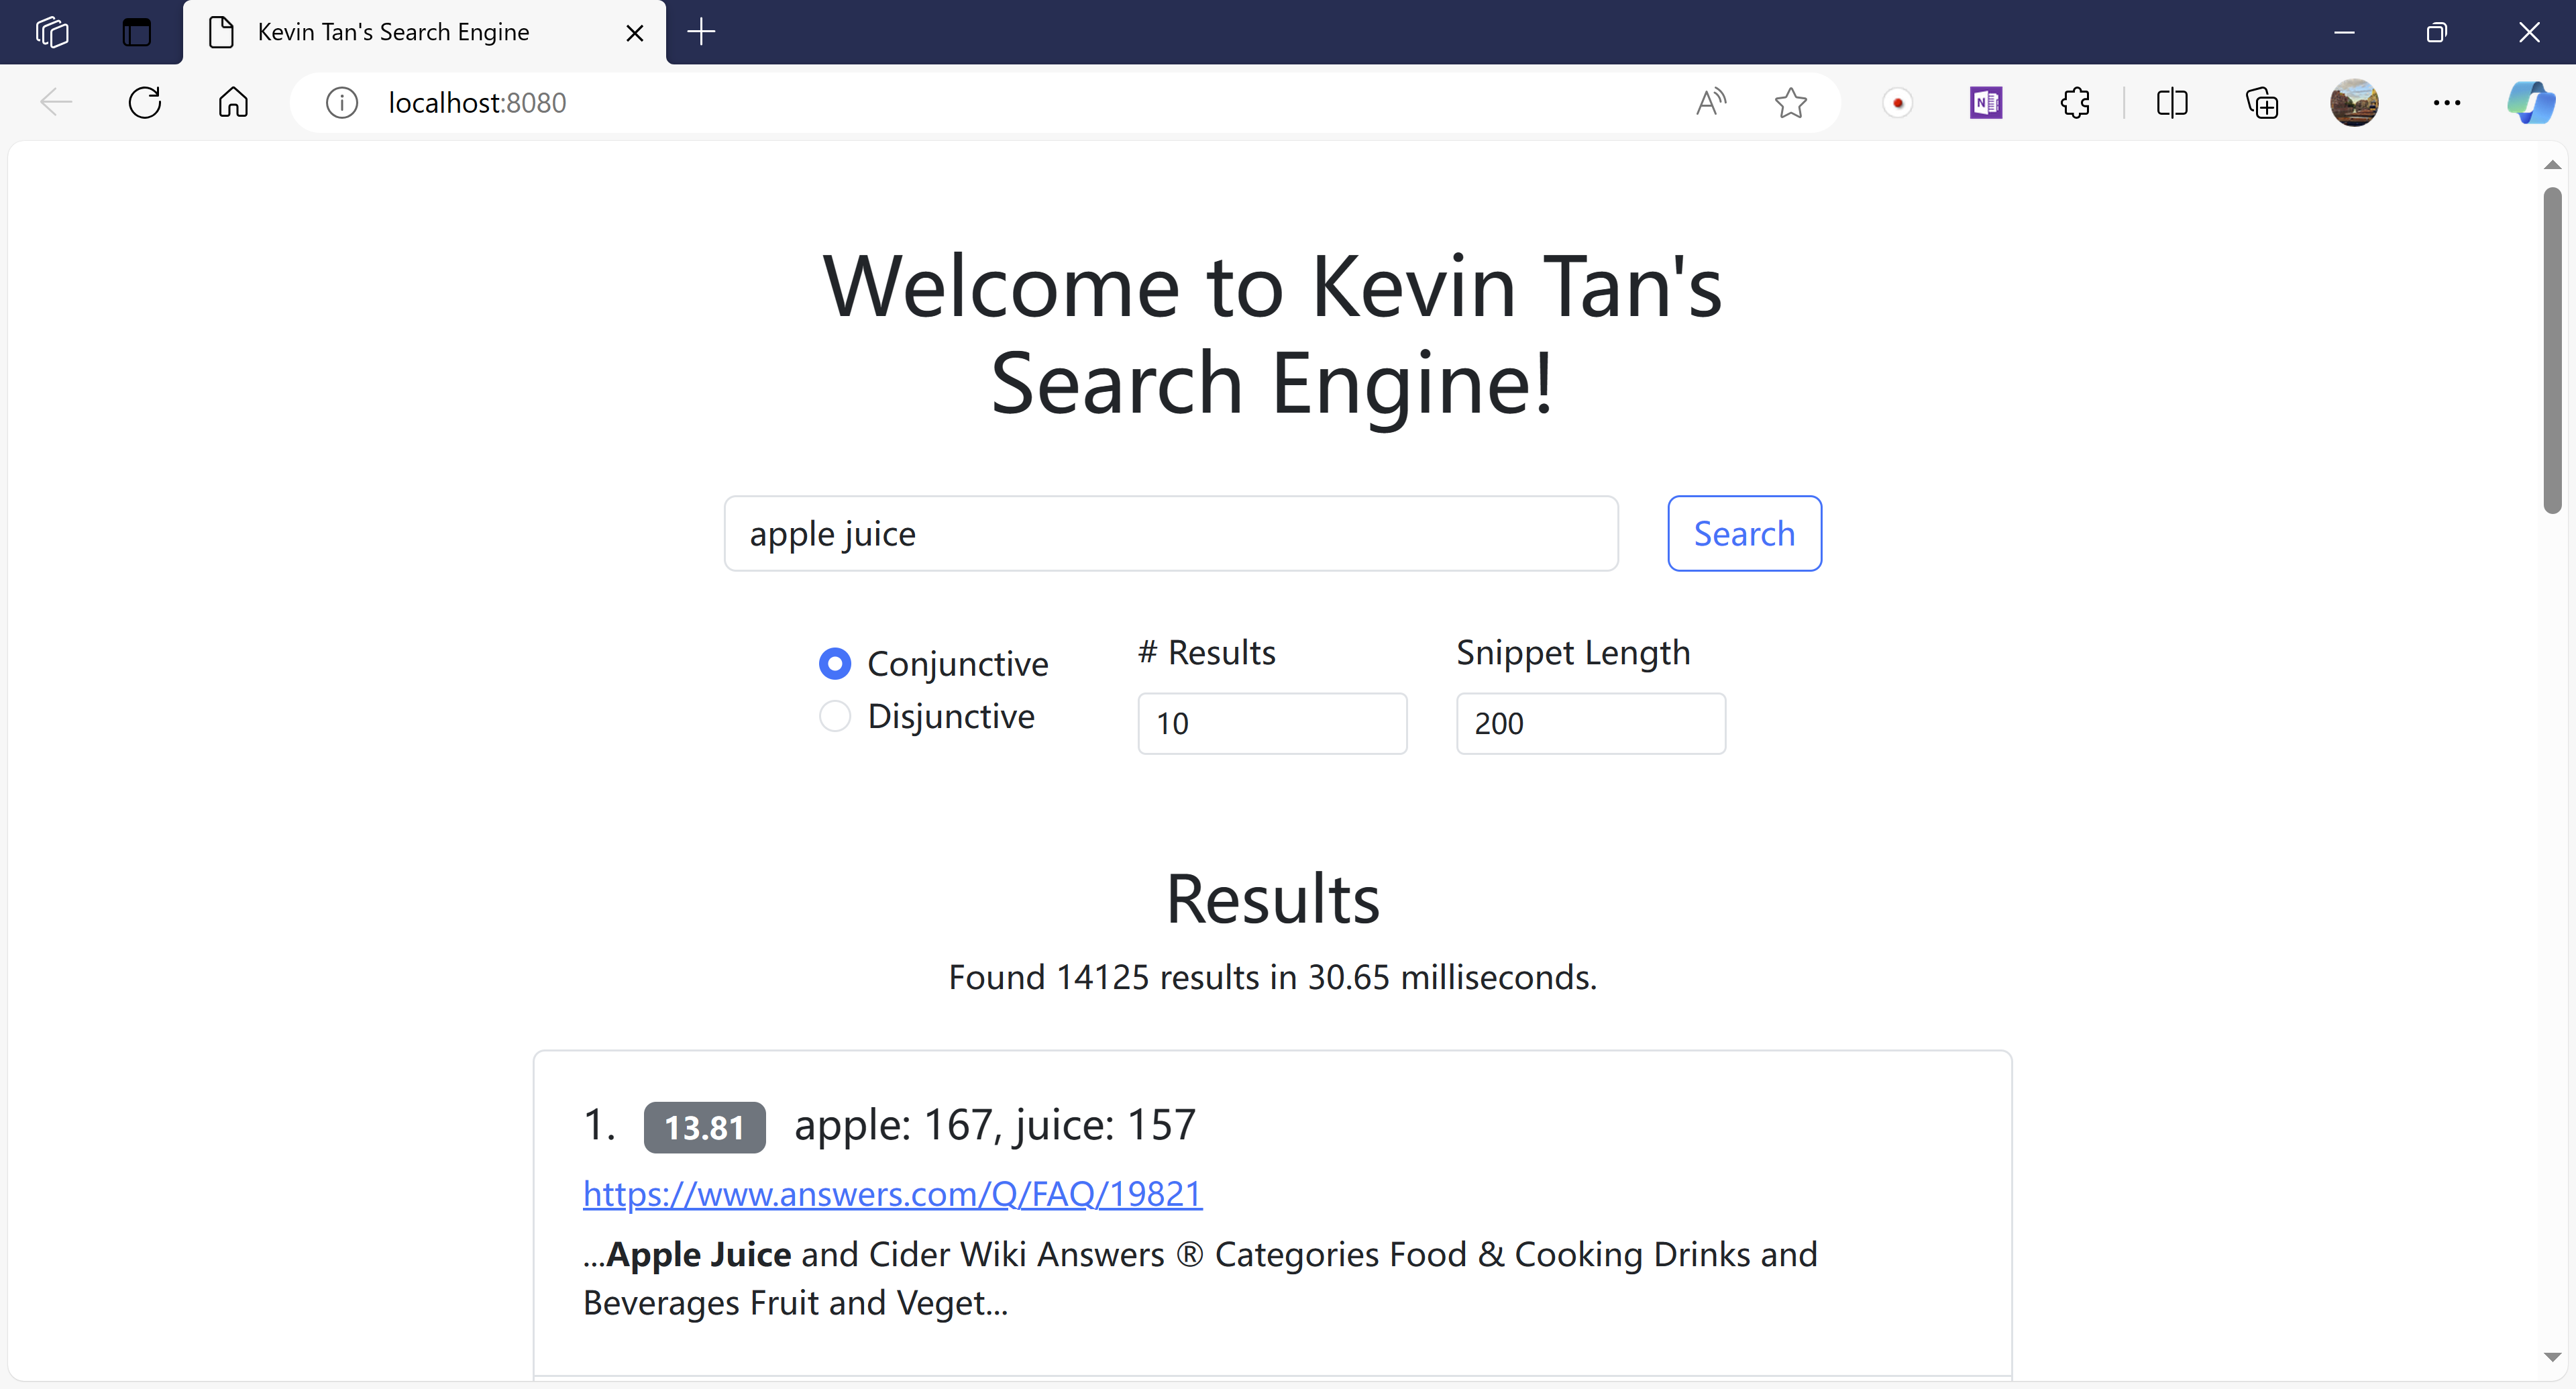
\includegraphics{readme.assets/image-20231112214558198.png}
\caption{A Mini Web Search Engine}
\label{conjunctive}
\end{figure}

\hypertarget{i-overview}{%
\section{I. Overview}\label{i-overview}}

Ostensibly, a search engine receives a user's input and then finds
relevant results to return to the user. However, it must achieve high
efficiency with limited resources, especially memory and disk space.
Unlike the usual space-for-time algorithms, the trade-off between time
and space must be considered everywhere when implementing a search
engine, as the data sets are large, and even trading time for space is
required.

The search engine needs to complete the following tasks to achieve the
desired functionality:

\begin{enumerate}
\def\labelenumi{\arabic{enumi}.}
\item
  Indexing a large dataset into an inverted index, which is basically a
  table with terms being the key and information related to the term
  being its value. Such information includes IDs of documents that
  contain the term and frequencies of the term in each document. Note
  that the index may be very large, so it is first generated in sorted
  chunks and then merged. During indexing, the dataset is tokenized to
  determine the boundaries of each term.
\item
  Preparing auxiliary data structures to speed up the query, including a
  table of document information, such as URL, number of terms, begin and
  end positions in the dataset, and a table of storage information
  (lexicon), which contains each term's start position in the index and
  number of documents containing the word.
\item
  Receiving and cleaning the query. The query may have leading and
  trailing blanks, repeated terms, consecutive blanks, and a mix of
  upper and lower case letters.
\item
  Checking if the query result is in the cache. If it is, return the
  cached result.
\item
  Getting the storage information from the lexicon and reading entries
  of query terms from the index file.
\item
  Selecting documents based on the query type, conjunctive or
  disjunctive.
\item
  Calculating the ranking score of the selected documents and sorting
  the results based on the score.
\item
  Caching the result.
\item
  Generating snippets of the result.
\item
  Returning the result.
\end{enumerate}

\hypertarget{ii-details}{%
\section{II. Details}\label{ii-details}}

The search engine contains three programs that create an inverted index
from the \texttt{msmarco-\\docs.trec.gz} dataset and process user's query
from the web or the command line.

\hypertarget{1-language}{%
\subsection{1. Language}\label{1-language}}

All the programs are written in the new standard of C++. A modern C++
compiler that supports the C++17 (maybe) standard is needed to compile
the programs. The programs are tested on Windows and may work on
Unix-based systems without modifying any code.

\hypertarget{2-disk-based-index-structures}{%
\subsection{2. Disk-based Index
Structures}\label{2-disk-based-index-structures}}

The programs create the following four files at the end, where
\texttt{\textless{}type\textgreater{}} is among \texttt{txt},
\texttt{bin}, and \texttt{vbyte}, corresponding to different supported
formats.

\begin{itemize}
\item
  \texttt{merged\_index.\textless{}type\textgreater{}}: The inverted
  index.
\item
  \texttt{freqs.\textless{}type\textgreater{}}: The frequencies of each
  term in each document.
\item
  \texttt{docs.txt}: The page table for looking up the URL, the number
  of terms, and the start and end position in the dataset of a document
  given its \texttt{docID}.
\item
  \texttt{storage\_\textless{}type\textgreater{}.txt}: The lexicon, a
  table for positioning a term's start position in the inverted index
  and the frequency file and looking up the number of docs containing
  the word.
\end{itemize}

\hypertarget{3-problem-decomposition}{%
\subsection{3. Problem Decomposition}\label{3-problem-decomposition}}

The first program, \texttt{create\_index}, reads the dataset into memory
by chunks, parses the dataset, creates the sorted inverted index and
frequency file for each chunk, and prepares the page table.

The second program, \texttt{merge\_index}, reads the inverted index and
frequency file created by the first program by chunks, merges them by a
\(k\)-way merge sort, and prepares the lexicon.

The third program, \texttt{main}, performs the query task. It is also a
web server in the web mode.

All programs are designed to be I/O-efficient, i.e., they can run fast
when memory is limited.

\hypertarget{4-parsing}{%
\subsection{4. Parsing}\label{4-parsing}}

Since HTML has already been removed, the dataset is parsed from scratch.
No parsing library is needed.

\hypertarget{5-data-format}{%
\subsection{5. Data Format}\label{5-data-format}}

The first program supports both the \texttt{gzip}-compressed format and
the uncompressed format. \texttt{zlib} library is built from source and
dynamically linked to the first program when it starts on Windows. On
Unix-based systems, you may install \texttt{zlib} using a package
manager and tell \texttt{cmake} to automatically find and link the
library in the \texttt{CMakeLists.txt} more elegantly. The program
automatically detects whether the dataset is compressed or not.

The third program could trivially support the \texttt{gzip}-compressed
format, but considering efficiency, it is currently not supported.

\hypertarget{6-index-file-format}{%
\subsection{6. Index File Format}\label{6-index-file-format}}

The supported formats of \textbf{temporary small chunks of index} files
created by the first program are as follows:

\begin{itemize}
\item
  \texttt{.txt} file: The human-readable text format for debugging. Each
  entry takes up one line containing the term and its \texttt{docID}s or
  frequencies, separated by a space.
\item
  \texttt{.bin} file: The uncompressed binary format. Each entry starts
  with the term, followed by a space, then by \texttt{docID}s, then by
  an \texttt{unsigned\ int} indicating the number of \texttt{docID}s.
  The rest of the entry is compressed \texttt{docID}s. Each
  \texttt{docID} takes up \texttt{sizeof(unsigned)} bytes, which is
  typically 4 bytes. For frequency files, they are the same as above,
  except that there is no need to store term strings.
\item
  \textbf{\texttt{.vbyte} file: The same as above, except that all
  \texttt{docID}s and frequencies are stored in a compressed format
  using the \texttt{vbyte} algorithm.}
\end{itemize}

The supported formats of the \textbf{final merged index} created by the
second program are as follows:

\begin{itemize}
\item
  \texttt{.txt} file: The same as above. \texttt{docID}s in each term
  can be stored in difference to save storage.
\item
  \texttt{.bin} file: The uncompressed binary format. All
  \texttt{docID}s are stored consecutively. \texttt{docID}s in each term
  can be stored in difference. The start position and number of
  documents of each entry are indicated by the lexicon. Each
  \texttt{docID} takes up \texttt{sizeof(unsigned)} bytes, which is
  typically 4 bytes. For frequency files, they are the same as above,
  except that there is no need to store differences.
\item
  \textbf{\texttt{.vbyte} file: The same as above, except that all
  \texttt{docID}s and frequencies are stored in a compressed format
  using the \texttt{vbyte} algorithm.} For frequency files, there is no
  need to store differences to achieve a high compression rate because
  frequencies are relatively small.
\end{itemize}

\hypertarget{7-docids-and-terms}{%
\subsection{\texorpdfstring{7. \texttt{DocID}s and
Terms}{7. DocIDs and Terms}}\label{7-docids-and-terms}}

\texttt{DocID}s are assigned in the order in which the pages are parsed,
so the page table does not need to store the \texttt{docID}s. Terms are
kept in textual format, and the final inverted lists do not have terms
inside each posting.

\hypertarget{8-unicode}{%
\subsection{8. Unicode}\label{8-unicode}}

Everything is kept using the UTF-8 encoding to save memory. When
parsing, if a character is within the ASCII range, \texttt{isalnum} is
used to determine word boundaries. Otherwise, only ``General
Punctuation'' (UTF-8 \texttt{0xE28080}--\texttt{0xE280AF}) and ``CJK
Symbols and Punctuation'' (UTF-8 \texttt{0xE38080}--\texttt{0xE381BF}) of
the Unicode blocks are regarded as word boundaries because Unicode has
so many symbols and invisible characters that should probably be part of
the word. Characters not in the ASCII range are not converted to
``lower'' cases because it may have drawbacks for many languages.

\hypertarget{9-query-execution}{%
\subsection{9. Query Execution}\label{9-query-execution}}

For extendibility and maintainability, the code uses STL and the new
standard of C++. Thus, the interface for accessing inverted lists at an
intermediate level in the architecture has different function names and
signatures from those introduced in the slides while hiding details such
as file input and inverted list compression techniques from the
higher-level query processor.

\hypertarget{10-ranked-queries}{%
\subsection{10. Ranked Queries}\label{10-ranked-queries}}

The program computes ranked queries according to the BM25 formula \cite{c1}

\begin{align}
\operatorname{BM25}(d, q) &= \sum_{t \in q} \operatorname{IDF}(t) \cdot \operatorname{TF}(d, t), \\
\operatorname{IDF}(t) &= \log \left(\frac{N-f_t+0.5}{f_t+0.5}\right), \\
\operatorname{TF}(d, t) &= \frac{f_{d, t} \cdot\left(k_1+1\right)}{f_{d, t}+k_1 \cdot\left(1-b+b \cdot l_d / l_{\mathrm{avg}}\right)},
\end{align}

where \(d\) is the document, \(q\) is the query, \(N\) is the number of
documents in the collection, \(f_t\) is the document frequency of term
\(t\), \(f_{d,t}\) is the frequency of \(t\) in \(d\), \(l_d\) is the
length of document \(d\), and \(l_\text{avg}\) is the average document
length. Parameters are set to be \(k_1 = 0.9\) and \(b = 0.4\), as
described by Trotman et al. \cite{c2}.

The top \(n\) results are returned according to the scoring function,
where \(n\) is defaulted to be 10 and can be set via command line
arguments or the web page. For each top result, its score according to
the ranking function and the frequency of each search term in the
document are returned. Conjunctive and disjunctive queries are
implemented, which can also be chosen via command line arguments or the
web page.

\hypertarget{11-interface}{%
\subsection{11. Interface}\label{11-interface}}

A responsive web page is built, which is shown in Fig. \ref{conjunctive} and Fig. \ref{web}.
Users can choose query type (conjunctive or disjunctive), number of
results, and snippet length. The query words are bolded in the snippet.
Ranking scores and query word frequencies are displayed. The web page is
responsive in extreme cases and renders according to the browser's color
theme. Querying multilingual words is supported.

Users can also access via the command line, which is shown in Fig. \ref{cli}.
Users can choose query type (conjunctive or disjunctive), number of
results, and snippet length via command line arguments. Ranking scores
and query word frequencies are displayed. Querying multilingual words is
only supported if the terminal is UTF-8 encoded.

\begin{figure}[!h]
  \begin{subfigure}{0.123\textwidth}
    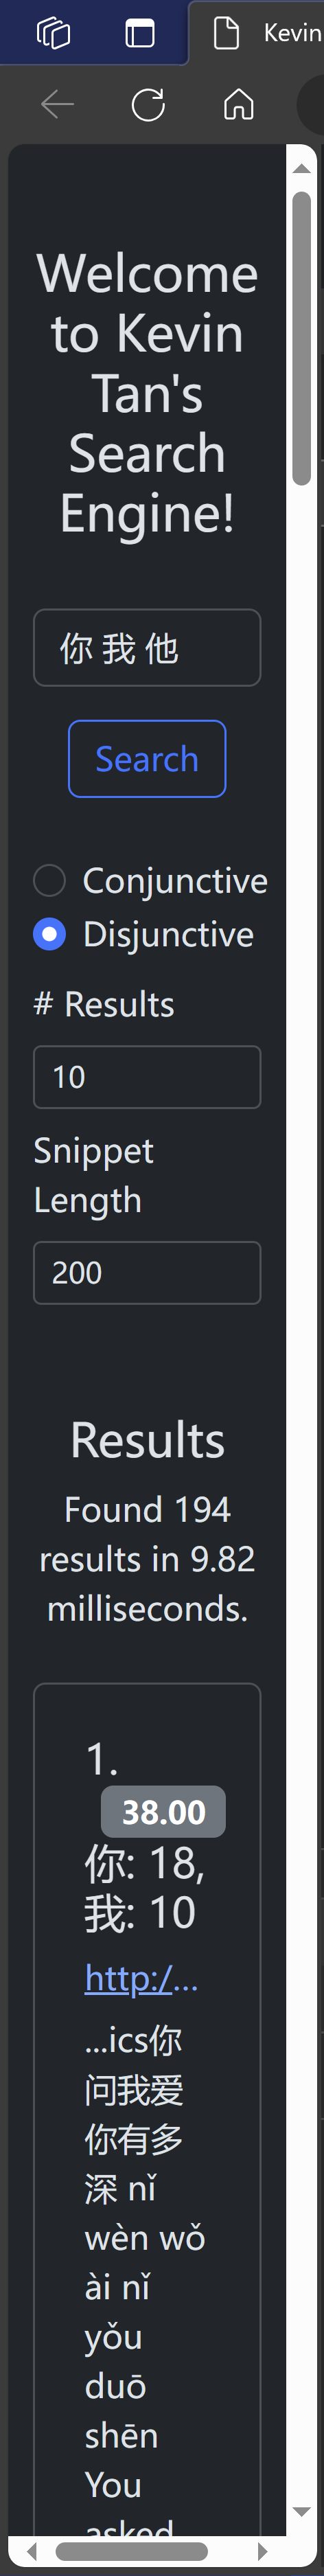
\includegraphics{readme.assets/image-20231112214917007.png}
    \caption{}
    \label{web}
  \end{subfigure}
  \begin{subfigure}{0.877\textwidth}
    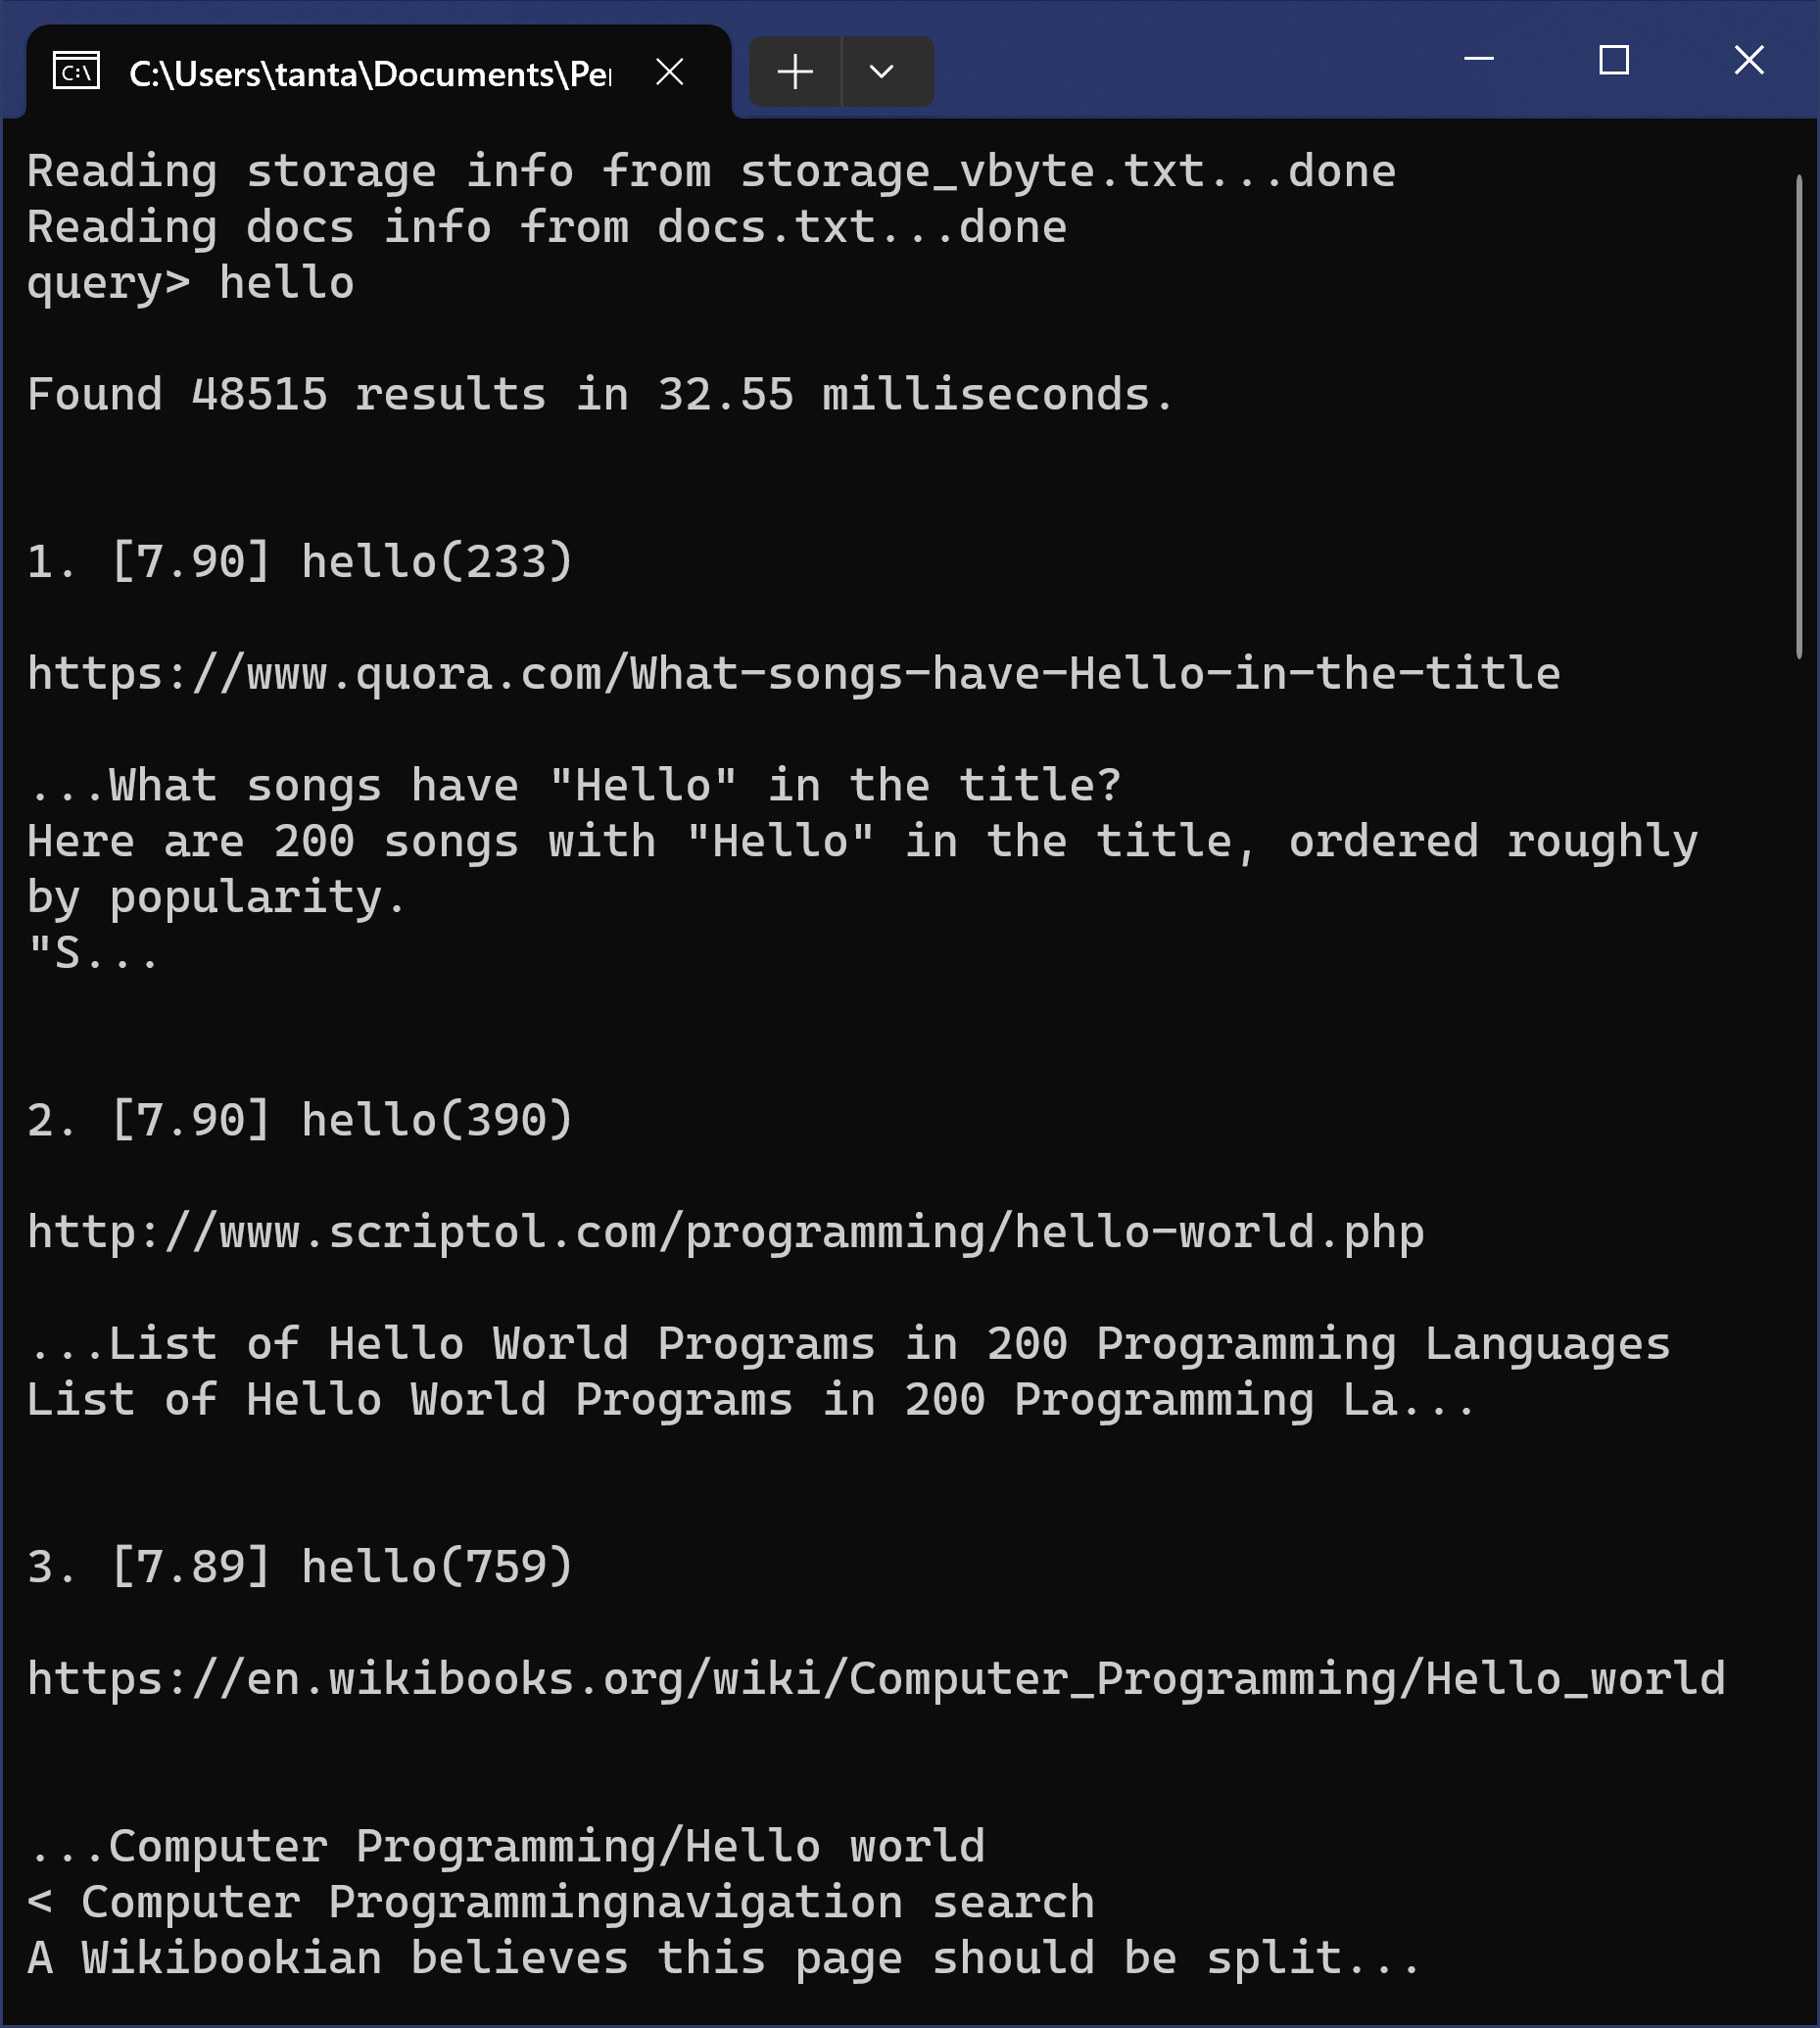
\includegraphics{readme.assets/image-20231112215534145.png}
    \caption{}
    \label{cli}
  \end{subfigure}
  \caption{The responsive web page supporting multilingual queries and the command line interface}
  \label{interfaces}
\end{figure}

Users can press \texttt{Ctrl-C} to exit the program. Resources are
released during exit.

\hypertarget{12-startup}{%
\subsection{12. Startup}\label{12-startup}}

Upon startup, the query processor reads the complete lexicon and page
table from disk into main memory. After the user inputs a query, the
program then seeks the file to read only those inverted lists that
correspond to query words and then computes the result. After returning
the result, the program waits for the next query to be input.
\textbf{Caching is implemented} using LRU caches. The amount of memory
that is used for index caching can be set via a command line argument.

\hypertarget{13-index-compression}{%
\subsection{13. Index Compression}\label{13-index-compression}}

The program supports inverted index in binary format and
\texttt{vbyte}-compressed format. For the latter, it is only
uncompressed on demand.

\hypertarget{iii-how-to-run-the-programs}{%
\section{III. How to Run the
Programs}\label{iii-how-to-run-the-programs}}

\hypertarget{1-createindex}{%
\subsection{\texorpdfstring{1.
\texttt{create\_index}}{1. create\_index}}\label{1-createindex}}

On Windows, please make sure \texttt{zlibwapi.dll} and
\texttt{create\_index.exe} are in the same directory.

\begin{Shaded}
\begin{Highlighting}[]
\ExtensionTok{Usage:}\NormalTok{ ./create\_index [{-}h] [{-}d dataset\_file\_path] [{-}i index\_path] [{-}p doc\_info\_path]}
        \ExtensionTok{[{-}t}\NormalTok{ index\_type] [{-}b input\_buffer\_size] [{-}e output\_entry\_size]}
\ExtensionTok{Options:}
        \ExtensionTok{{-}d}\NormalTok{      dataset path, default: msmarco{-}docs.trec.gz}
        \ExtensionTok{{-}i}\NormalTok{      index path, default: index}
        \ExtensionTok{{-}p}\NormalTok{      doc info }\ErrorTok{(}\ExtensionTok{page}\NormalTok{ table}\KeywordTok{)} \ExtensionTok{path,}\NormalTok{ default: .}
        \ExtensionTok{{-}t}\NormalTok{      index type }\ErrorTok{(}\ExtensionTok{txt}\KeywordTok{|}\ExtensionTok{bin}\KeywordTok{|}\ExtensionTok{vbyte}\KeywordTok{)}\ExtensionTok{,}\NormalTok{ default: vbyte}
        \ExtensionTok{{-}b}\NormalTok{      input buffer size }\ErrorTok{(}\ExtensionTok{unsigned}\NormalTok{ int but must }\OperatorTok{\textless{}}\NormalTok{ 2GB, unit: bytes}\KeywordTok{)}\ExtensionTok{,}
                \ExtensionTok{default:}\NormalTok{ 256MB}
        \ExtensionTok{{-}e}\NormalTok{      output entry size, default: 1000000}
        \ExtensionTok{{-}h}\NormalTok{      help}
\end{Highlighting}
\end{Shaded}

\hypertarget{2-mergeindex}{%
\subsection{\texorpdfstring{2.
\texttt{merge\_index}}{2. merge\_index}}\label{2-mergeindex}}

\begin{Shaded}
\begin{Highlighting}[]
\ExtensionTok{Usage:}\NormalTok{ ./merge\_index [{-}h] [{-}i index\_path] [{-}s storage\_path] [{-}o merged\_index\_path]}
        \ExtensionTok{[{-}t}\NormalTok{ input\_index\_type] [{-}m merged\_index\_type] [{-}d store\_diff]}
        \ExtensionTok{[{-}c}\NormalTok{ input\_index\_chunk\_size] [{-}e output\_entry\_size]}
\ExtensionTok{Options:}
        \ExtensionTok{{-}i}\NormalTok{      index path, default: index}
        \ExtensionTok{{-}s}\NormalTok{      storage info }\ErrorTok{(}\ExtensionTok{lexicon}\KeywordTok{)} \ExtensionTok{path,}\NormalTok{ default: .}
        \ExtensionTok{{-}o}\NormalTok{      merged index path, default: .}
        \ExtensionTok{{-}t}\NormalTok{      input index type }\ErrorTok{(}\ExtensionTok{txt}\KeywordTok{|}\ExtensionTok{bin}\KeywordTok{|}\ExtensionTok{vbyte}\KeywordTok{)}\ExtensionTok{,}\NormalTok{ default: vbyte}
        \ExtensionTok{{-}m}\NormalTok{      merged index type }\ErrorTok{(}\ExtensionTok{txt}\KeywordTok{|}\ExtensionTok{bin}\KeywordTok{|}\ExtensionTok{vbyte}\KeywordTok{)}\ExtensionTok{,}\NormalTok{ default: vbyte}
        \ExtensionTok{{-}d}\NormalTok{      store diff docIDs in the merged index }\ErrorTok{(}\FunctionTok{true}\KeywordTok{|}\FunctionTok{false}\KeywordTok{)}\ExtensionTok{,}\NormalTok{ default: true}
        \ExtensionTok{{-}c}\NormalTok{      input index chunk size, default: 5000}
        \ExtensionTok{{-}e}\NormalTok{      output entry size, default: 100000}
        \ExtensionTok{{-}h}\NormalTok{      help}
\end{Highlighting}
\end{Shaded}

\hypertarget{3-main}{%
\subsection{\texorpdfstring{3.
\texttt{main}}{3. main}}\label{3-main}}

\begin{Shaded}
\begin{Highlighting}[]
\ExtensionTok{Usage:}\NormalTok{ ./main [{-}h] [{-}d dataset\_file] [{-}p doc\_info\_file] [{-}s storage\_info\_file]}
        \ExtensionTok{[{-}i}\NormalTok{ index\_ids\_file] [{-}f index\_freqs\_file] [{-}t index\_file\_type]}
        \ExtensionTok{[{-}w}\NormalTok{ server\_port] [{-}c conjunctive\_query] [{-}n n\_results] [{-}l snippet\_len]}
        \ExtensionTok{[{-}m}\NormalTok{ cache\_size]}
\ExtensionTok{Options:}
        \ExtensionTok{{-}d}\NormalTok{      dataset file, default: fulldocs{-}new.trec}
        \ExtensionTok{{-}p}\NormalTok{      doc info }\ErrorTok{(}\ExtensionTok{page}\NormalTok{ table}\KeywordTok{)} \FunctionTok{file}\NormalTok{, default: docs.txt}
        \ExtensionTok{{-}s}\NormalTok{      storage info }\ErrorTok{(}\ExtensionTok{lexicon}\KeywordTok{)} \FunctionTok{file}\NormalTok{, default: storage\_vbyte.txt}
        \ExtensionTok{{-}i}\NormalTok{      index ids file, default: merged\_index.vbyte}
        \ExtensionTok{{-}f}\NormalTok{      index freqs file, default: freqs.vbyte}
        \ExtensionTok{{-}t}\NormalTok{      index file type }\ErrorTok{(}\ExtensionTok{bin}\KeywordTok{|}\ExtensionTok{vbyte}\KeywordTok{)}\ExtensionTok{,}\NormalTok{ default: vbyte}
        \ExtensionTok{{-}w}\NormalTok{      server port }\ErrorTok{(}\ExtensionTok{[0,}\NormalTok{ 65535] for web, others for cli}\KeywordTok{)}\ExtensionTok{,}\NormalTok{ default: 8080}
        \ExtensionTok{{-}c}\NormalTok{      conjunctive query for cli }\ErrorTok{(}\FunctionTok{true}\KeywordTok{|}\FunctionTok{false}\KeywordTok{)}\ExtensionTok{,}\NormalTok{ default: true}
        \ExtensionTok{{-}n}\NormalTok{      number of results, default: 10}
        \ExtensionTok{{-}l}\NormalTok{      snippet length, default: 200}
        \ExtensionTok{{-}m}\NormalTok{      cache size, default: 1000}
        \ExtensionTok{{-}h}\NormalTok{      help}
\end{Highlighting}
\end{Shaded}

\hypertarget{iii-how-it-works-internally-design-decisions-limitations-and-major-parts}{%
\section{III. How It Works Internally, Design Decisions, Limitations,
and Major
Parts}\label{iii-how-it-works-internally-design-decisions-limitations-and-major-parts}}

The programs first set up default options and update them according to
the parsed command line input.

\hypertarget{1-createindex-2}{%
\subsection{\texorpdfstring{1.
\texttt{create\_index}}{1. create\_index}}\label{1-createindex-2}}

Then, it starts to read and parse the dataset.

When it comes to efficient I/O, the most efficient one should be memory
mapping, which avoids copying data between the kernel space and the user
space. The OS controls whether the data have been actually loaded into
the memory or written to the disk; no byte array is needed. In addition,
user-level data structures can only store pointers to the mapped memory
to represent corresponding strings rather than copy them. However, I was
asked not to use memory mapping for indexing. Then, the most efficient
I/O should be to read a chunk into a buffer, parse it until it reaches
the end, read another chunk, and so forth. Strings also have to be
copied because the buffer may be updated before the strings are used.

When indexing, \texttt{unordered\_map} is used, which is a Hash table
storing each term, its \texttt{docID}s, and the term's frequency in each
document. When its size reaches the \texttt{output\_entry\_size}, this
chunk of the index is sorted according to the terms and then written to
the disk. \texttt{DocID}s and frequencies are stored in separate files
for better maintainability and efficiency. This part of the page table
is also written to the disk. Although sorting an \texttt{unordered\_map}
requires \(O(n \log n)\) time, it is only needed before it is written to
disk and does not copy data since pointers are used. More operations are
\texttt{find} and \texttt{insert}, which take \(O(1)\) in
\texttt{unordered\_map} and \(O(\log n)\) in \texttt{map}. Thus,
\texttt{unordered\_map} should be more efficient. \texttt{vector}, a
dynamic array, is used to store the page table. Finally, all indexes and
the page table are written to the disk.

\hypertarget{2-mergeindex-2}{%
\subsection{\texorpdfstring{2.
\texttt{merge\_index}}{2. merge\_index}}\label{2-mergeindex-2}}

Then, it reads \texttt{input\_index\_chunk\_size} of each temporary
index file produced by \texttt{create\_index} and then pushes all the
first entries of these chunks and their sources into a
\texttt{priority\_queue}. The smallest entry gets out of the queue and
is appended to or merged into the last entry of the final index, which
is a \texttt{vector}, and the head entry of its source gets into the
queue. When a chunk is empty, new entries from the same source are
loaded. This is a \(k\)-way merge sort. When the final index reaches
\texttt{output\_entry\_size}, it is written to the disk and cleared to
save memory. Lexicon is recorded simultaneously and is written to the
disk and cleared to save memory after this chunk of the final index is
written to the disk and cleared. Ultimately, all indexes and the lexicon
are written to the disk.

Frequencies, not BM25 scores, are stored based on the following
considerations. First, BM25 scores are floats, so they must be quantized
for better compression. However, some scores are too close and may lose
accuracy if quantized. Second, calculating BM25 at indexing
significantly increases time usage, and since there are so many words
and articles, most of the calculation results will never be used.

\hypertarget{3-the-main-program-and-the-indexhtml-web-page}{%
\subsection{\texorpdfstring{3. The \texttt{main} program and the
\texttt{index.html} web
page}{3. The main program and the index.html web page}}\label{3-the-main-program-and-the-indexhtml-web-page}}

Then, it reads the page table and the lexicon into the memory and waits
for input from the user. After receiving the user's query, it cleans it,
removing leading and trailing blanks and repeated terms, and converts
ascii letters to lowercase letters. Then, it checks if the query result
is in the cache. If it is, it returns the cached result. Otherwise, it
checks if each term's index entry is in the cache. If not, it gets the
storage information from the lexicon and reads entries of query terms
from the index file. After that, it selects documents based on the query
type, conjunctive and disjunctive. Since \texttt{docID}s are sorted,
conjunctive query intersects \texttt{docID}s in \(O(n)\) time, and
disjunctive query unions \texttt{docID}s also in \(O(n)\) time. Then, it
calculates the ranking score of the selected documents using BM25 and
sorts them based on the score. The consideration here is the same as
\texttt{create\_index}. After that, it caches the result and generates
snippets of the result. It seeks the dataset according to the
information in the page table, tokenizes the document, finds the first
occurrence of one of the query terms, and expands the start and end
positions of the snippet according to this position. Since the snippet
length can be changed via the web API, there is no point in caching
snippets. Finally, it returns the results to the web or the terminal.
During the entire process, pointers are used to avoid copying arrays for
efficiency.

The single-header library \texttt{httplib.h} is used for the program to
become a web server. The server responds with \texttt{index.html} for
HTTP GET requests and JSON for HTTP POST requests to the root. The
server is robust to bad requests, including malformed JSON, missing
properties, type-mismatch, invalid values, etc. In \texttt{index.html},
Bootstrap is used to build the responsive UI, and \texttt{axios} is used
to send asynchronized HTTP POST requests to the server. Results are
dynamically added to the page using JavaScript.

An example of the JSON sent from the web is shown as follows:

\begin{Shaded}
\begin{Highlighting}[]
\FunctionTok{\{}
    \DataTypeTok{"query"}\FunctionTok{:} \StringTok{"\textless{}query words\textgreater{}"}\FunctionTok{,}
    \DataTypeTok{"conjunctive"}\FunctionTok{:} \KeywordTok{true}\FunctionTok{,}
    \DataTypeTok{"n\_results"}\FunctionTok{:} \DecValTok{10}\FunctionTok{,}
    \DataTypeTok{"snippet\_len"}\FunctionTok{:} \DecValTok{200}
\FunctionTok{\}}
\end{Highlighting}
\end{Shaded}

An example of a successful query of the JSON returned from the server is
shown as follows:

\begin{Shaded}
\begin{Highlighting}[]
\FunctionTok{\{}
    \DataTypeTok{"cached"}\FunctionTok{:} \KeywordTok{true}\FunctionTok{,}
    \DataTypeTok{"time"}\FunctionTok{:} \DecValTok{1}\FunctionTok{,} \ErrorTok{//} \ErrorTok{in} \ErrorTok{microseconds}
    \DataTypeTok{"count"}\FunctionTok{:} \DecValTok{10000}\FunctionTok{,}
    \DataTypeTok{"data"}\FunctionTok{:} \OtherTok{[}
        \FunctionTok{\{}
            \DataTypeTok{"rank"}\FunctionTok{:} \DecValTok{1}\FunctionTok{,}
            \DataTypeTok{"score"}\FunctionTok{:} \FloatTok{7.6}\FunctionTok{,}
            \DataTypeTok{"freqs"}\FunctionTok{:} \OtherTok{[[}\StringTok{"\textless{}a query word\textgreater{}"}\OtherTok{,} \DecValTok{1000}\OtherTok{],} \ErrorTok{/*...*/}\OtherTok{]}\FunctionTok{,}
            \DataTypeTok{"url"}\FunctionTok{:} \StringTok{"\textless{}url\textgreater{}"}
            \StringTok{"snippet"}\ErrorTok{:} \StringTok{"\textless{}snippet\textgreater{}"}
        \FunctionTok{\}}\OtherTok{,} \ErrorTok{//} \ErrorTok{...}
    \OtherTok{]}
\FunctionTok{\}}
\end{Highlighting}
\end{Shaded}

\hypertarget{4-common}{%
\subsection{4. Common}\label{4-common}}

There are no major limitations of the programs; however, there are
requirements for the input and the environment:

\begin{itemize}
\item
  The \texttt{output\_entry\_size} of \texttt{create\_index} cannot be
  too small. Otherwise, there will be too many index files to be merged,
  and thus, the maximum limit of simultaneous open files may be reached
  in \texttt{merge\_index}. No more than 253 files (actually 256 files,
  including \texttt{stdin}, \texttt{stdout}, and \texttt{stderr}) can be
  opened at the same time.
\item
  The \texttt{input\_buffer\_size} must be less than 2 GB because
  \texttt{gzread} returns \texttt{int}. If a buffer larger than 2 GB is
  needed without memory mapping, more code will be involved, but the
  program does not require so much memory.
\item
  The dataset should not have more than \(2^{32}\) documents because
  \texttt{doc\_cnt} is an \texttt{unsigned\ int}. Each document cannot
  have more than \(2^{32}\) terms because \texttt{term\_cnt} is an
  \texttt{unsigned\ int}. They could be \texttt{size\_t}, but then it
  would take up more memory.
\item
  The dataset should not contain UTF-8 characters with more than 4 bytes
  because they are rare, and \texttt{msmarco-docs.trec.gz} does not have
  them.
\item
  The line break of text files should not be
  \texttt{\textbackslash{}r\textbackslash{}n} because
  \texttt{msmarco-docs.trec.gz} uses \texttt{\textbackslash{}n}, and it
  would be more inefficient to detect \texttt{\textbackslash{}r} when
  parsing such large files.
\item
  Binary files produced by the programs cannot be shared across
  processors with different endian. Most processors have the same
  endian, and it would be more inefficient to detect endianness in the
  program that processes such large files.
\item
  The web server is not designed to receive concurrent queries.
  This decision keeps the program lightweight.
\end{itemize}

\hypertarget{iv-results}{%
\section{IV. Results}\label{iv-results}}

The programs run on a laptop with an i7-9750H CPU clocked at 2.9 GHz and
64 GB RAM. The programs are compiled using the MSVC compiler. The
performance is subject to the status of the computer at that time. They
will run much faster on newer platforms and Unix-based systems.

\hypertarget{1-createindex-3}{%
\subsection{\texorpdfstring{1.
\texttt{create\_index}}{1. create\_index}}\label{1-createindex-3}}

With default options, the program takes almost 19 minutes to produce 75
chunks of temporary index files with less than 90 MB each. The page table
is 217 MB with 3213835 documents. The peak of the memory use is 686 MB, as
shown in Fig. \ref{create_vbyte_zipped}.

\begin{figure}
  \centering
  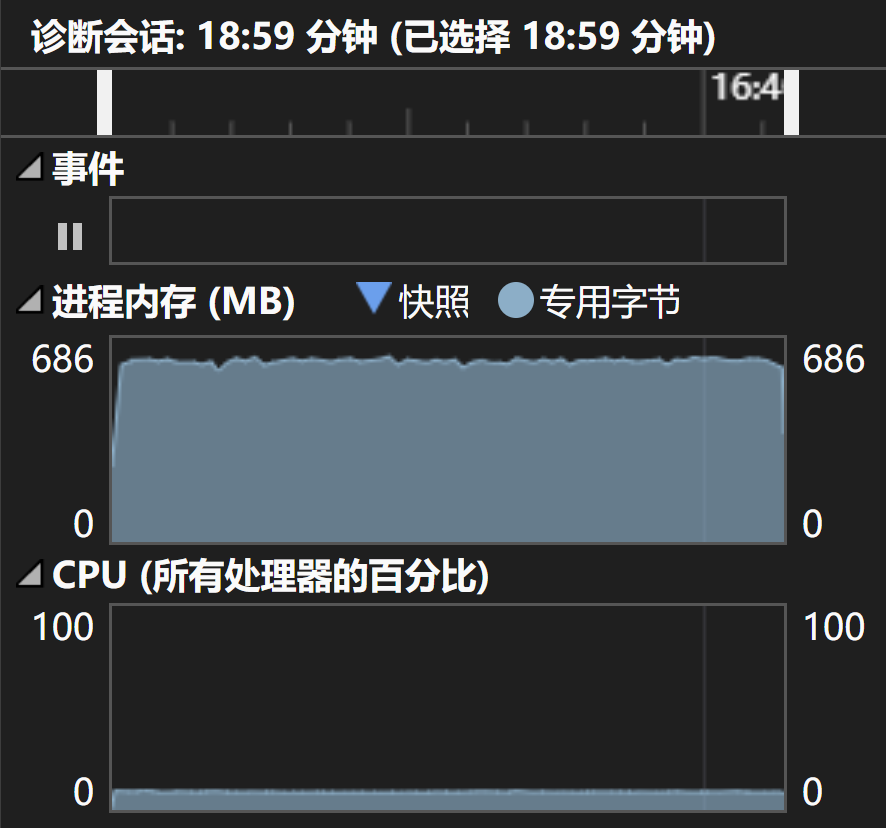
\includegraphics[width=0.5\textwidth]{readme.assets/image-20231107015648204.png}
  \caption{Time and memory usage of \texttt{create\_index} with
  default options}
  \label{create_vbyte_zipped}
\end{figure}

With default options, except that we directly read the uncompressed
dataset, the program takes almost 17 minutes to produce the files. The
peak of the memory use is 686 MB, as shown in Fig. \ref{create_vbyte}. Uncompressing in
advance saves about one minute.

\begin{figure}[!h]
  \centering
  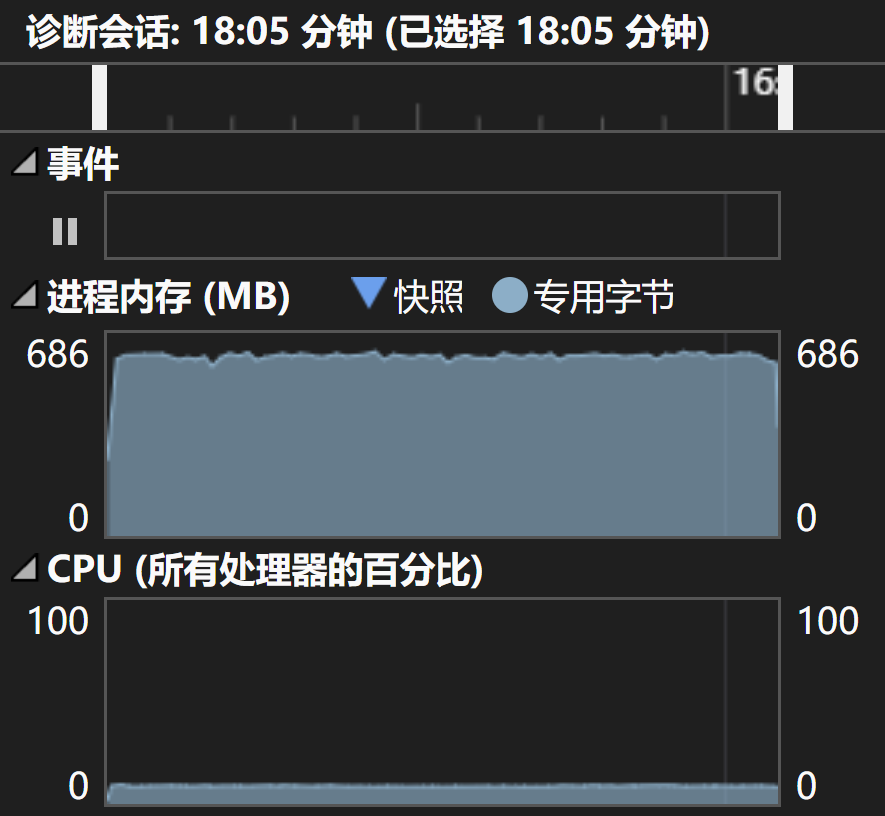
\includegraphics[width=0.5\textwidth]{readme.assets/image-20231107051503452.png}
  \caption{Time and memory usage of \texttt{create\_index} with default options but uncompressed dataset}
  \label{create_vbyte}
\end{figure}

If \texttt{bin} is used instead of \texttt{vbyte} in default options and
we directly read the uncompressed dataset, the program also takes almost
17 minutes to produce the files. The peak of the memory use is also 686
MB, as shown in Fig. \ref{create_bin}. \texttt{vbyte} compression consumes about one more
minute.

\begin{figure}[!h]
  \centering
  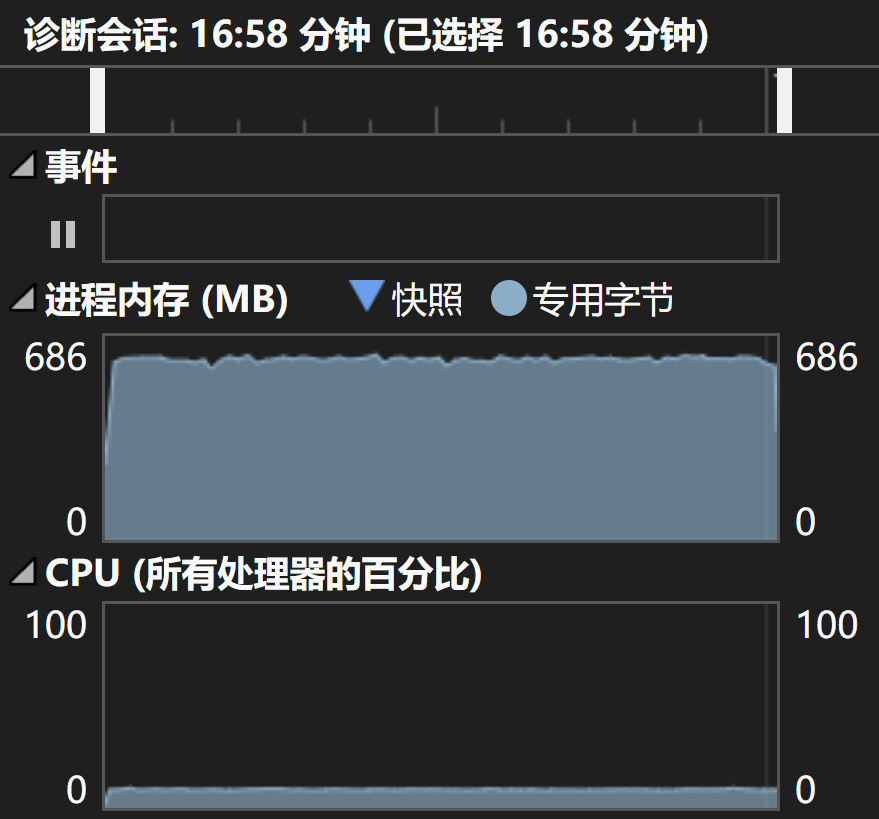
\includegraphics[width=0.5\textwidth]{readme.assets/create_bin-1699316895867-4.png}
  \caption{Time and memory usage of \texttt{create\_index} with default options but uncompressed dataset and \texttt{bin} files}
  \label{create_bin}
\end{figure}

\hypertarget{2-mergeindex-3}{%
\subsection{\texorpdfstring{2.
\texttt{merge\_index}}{2. merge\_index}}\label{2-mergeindex-3}}

With default options, the program takes 9 minutes and 27 seconds to
produce the final index file of 1.52 GB and the frequency file of 1.17
GB, with 25236693 entries and a lexicon of 840 MB. The peak of the
memory use is 417 MB, with an average of around 200 MB, as shown in Fig. \ref{merge_vbyte}.

\begin{figure}[!h]
  \centering
  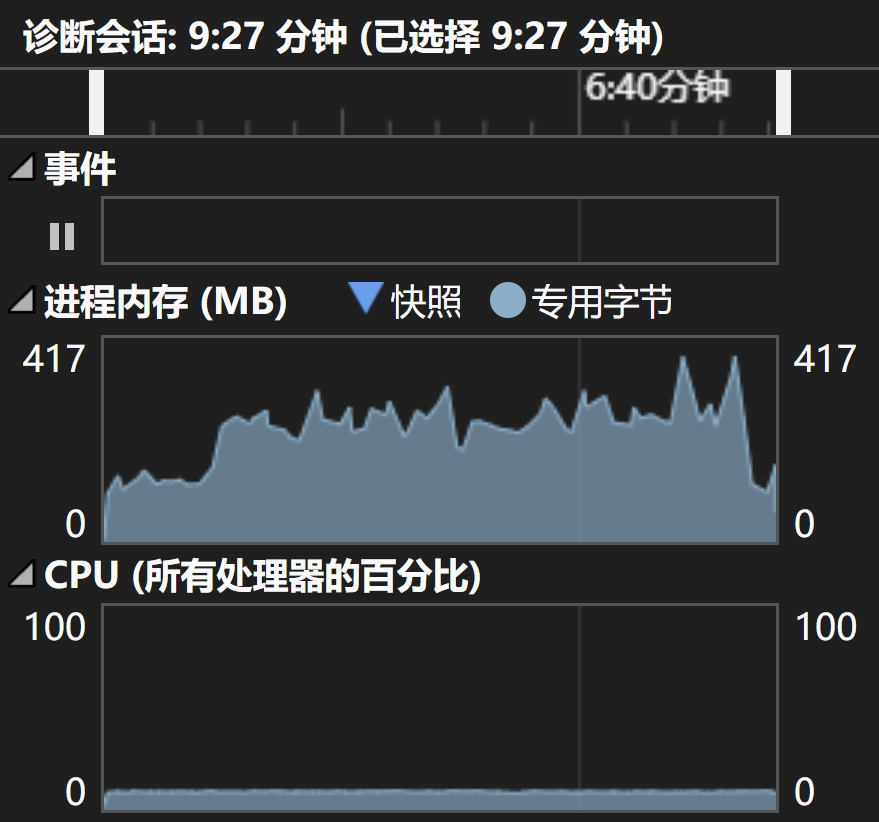
\includegraphics[width=0.5\textwidth]{readme.assets/merge_vbyte-1699317018747-6.png}
  \vspace{-4pt}
  \caption{Time and memory usage of \texttt{merge\_index} with default options}
  \label{merge_vbyte}
  \vspace{-4pt}
\end{figure}

If \texttt{bin} is used instead of \texttt{vbyte}, the program takes 6
minutes and 15 seconds to produce the final index file and the frequency
file of 4.69 GB for each, with a lexicon of 865 MB. The peak of the
memory use is 416 MB, with an average of around 200 MB, as shown in Fig. \ref{merge_bin}.

\begin{figure}[!h]
  \centering
  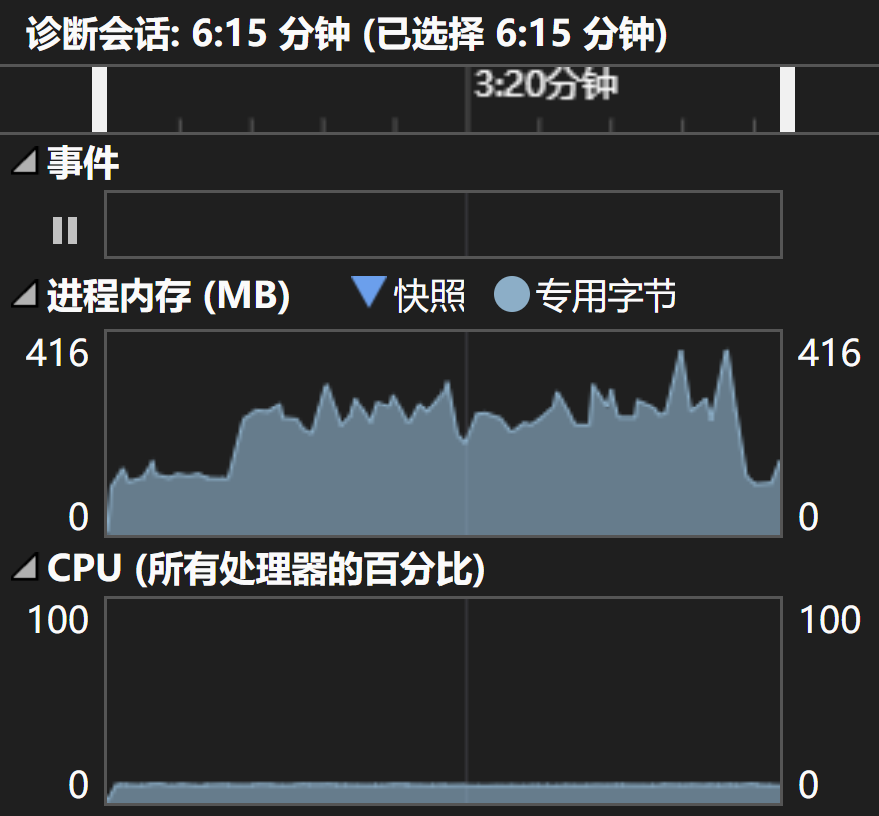
\includegraphics{readme.assets/merge_bin-1699317091540-8.png}
  \vspace{-4pt}
  \caption{Time and memory usage of \texttt{merge\_index} with default options but \texttt{bin} files}
  \label{merge_bin}
  \vspace{-4pt}
\end{figure}

The compression rate for the index file is

\[\frac{1.52}{4.69} \times 100\% \approx 32.4\%.\]

The compression rate for the frequency file is

\[\frac{1.17}{4.69} \times 100\% \approx 24.9\%.\]

If raw \texttt{docID}s are stored instead of the differences, the final
index file will be 3.92 GB, which does not have a good compression rate.
However, since word frequencies are relatively small, storing raw
frequencies already has a good compression rate.

\hypertarget{3-main-2}{%
\subsection{\texorpdfstring{3.
\texttt{main}}{3. main}}\label{3-main-2}}

New queries can be executed typically in tens to hundreds of
milliseconds, as shown in Fig. \ref{conjunctive} and Fig. \ref{interfaces}. Cached results can be
fetched in several microseconds, as shown in Fig. \ref{cached}.

\begin{figure}[!h]
  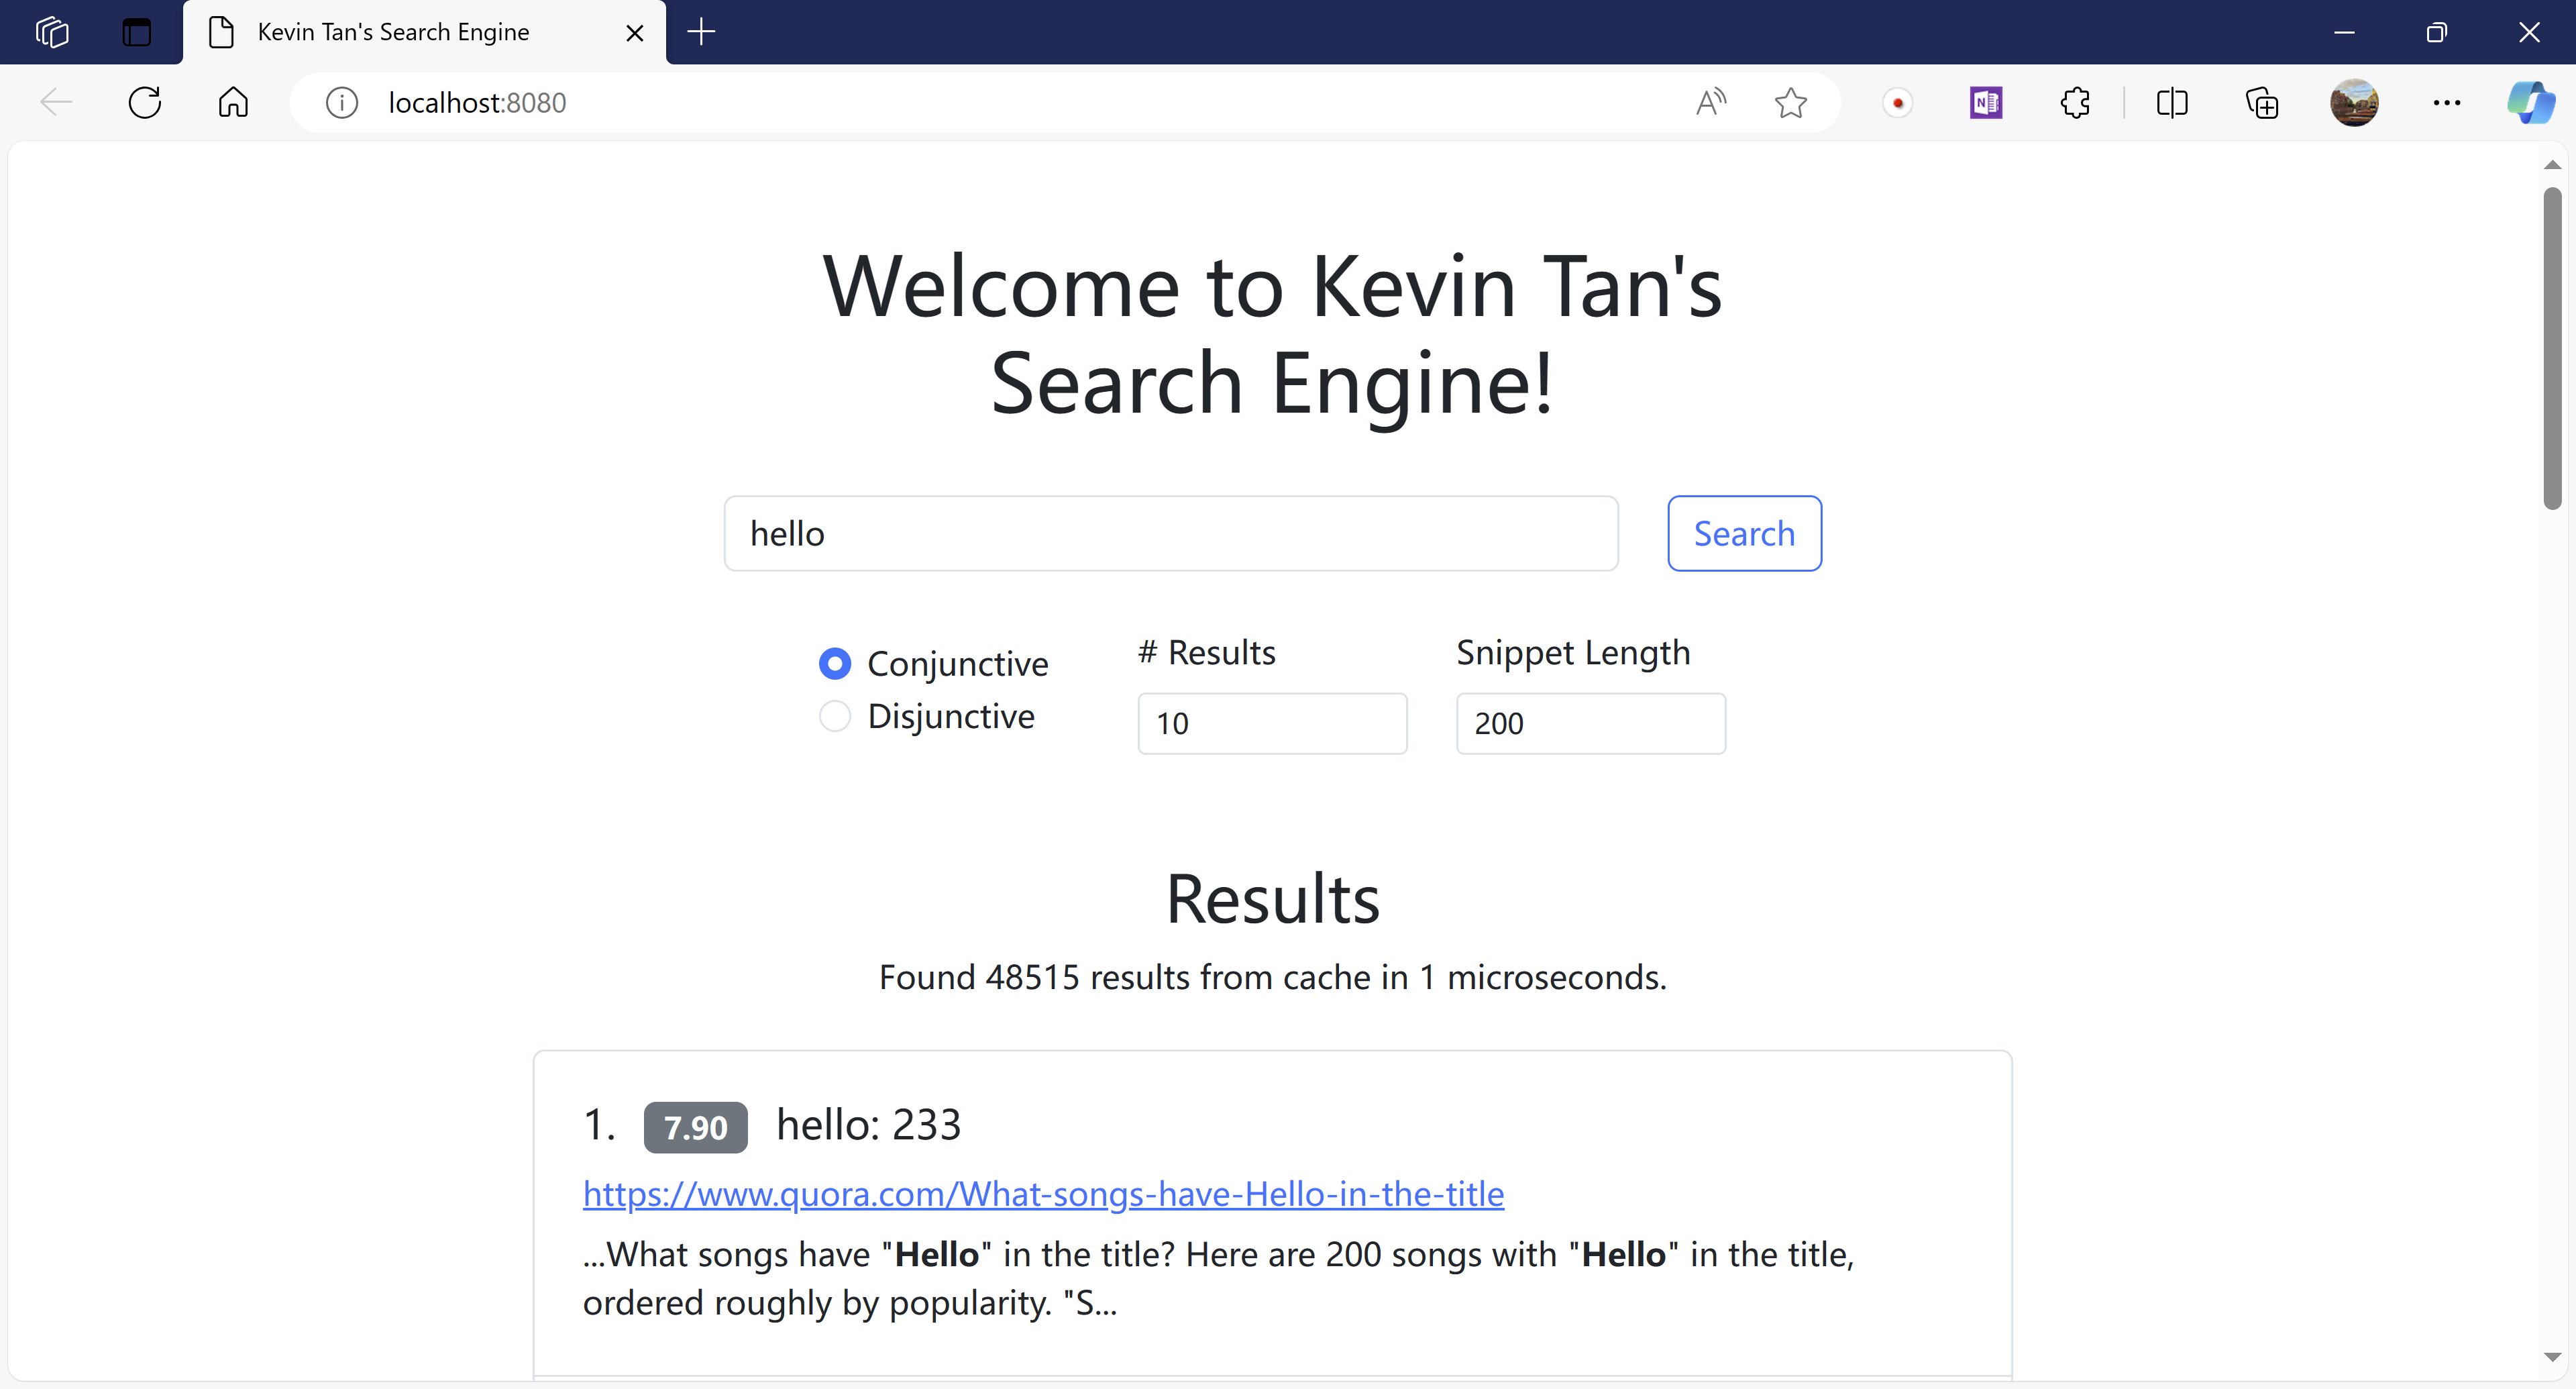
\includegraphics{readme.assets/image-20231112215219633.png}
  \vspace{-8pt}
  \caption{Cached query results can be fetched in several microseconds}
  \label{cached}
\end{figure}

Conjunctive queries typically cost less time than disjunctive queries,
as shown in Fig. \ref{conjunctive} and Fig. \ref{disjunctive}.

\begin{figure}[!h]
  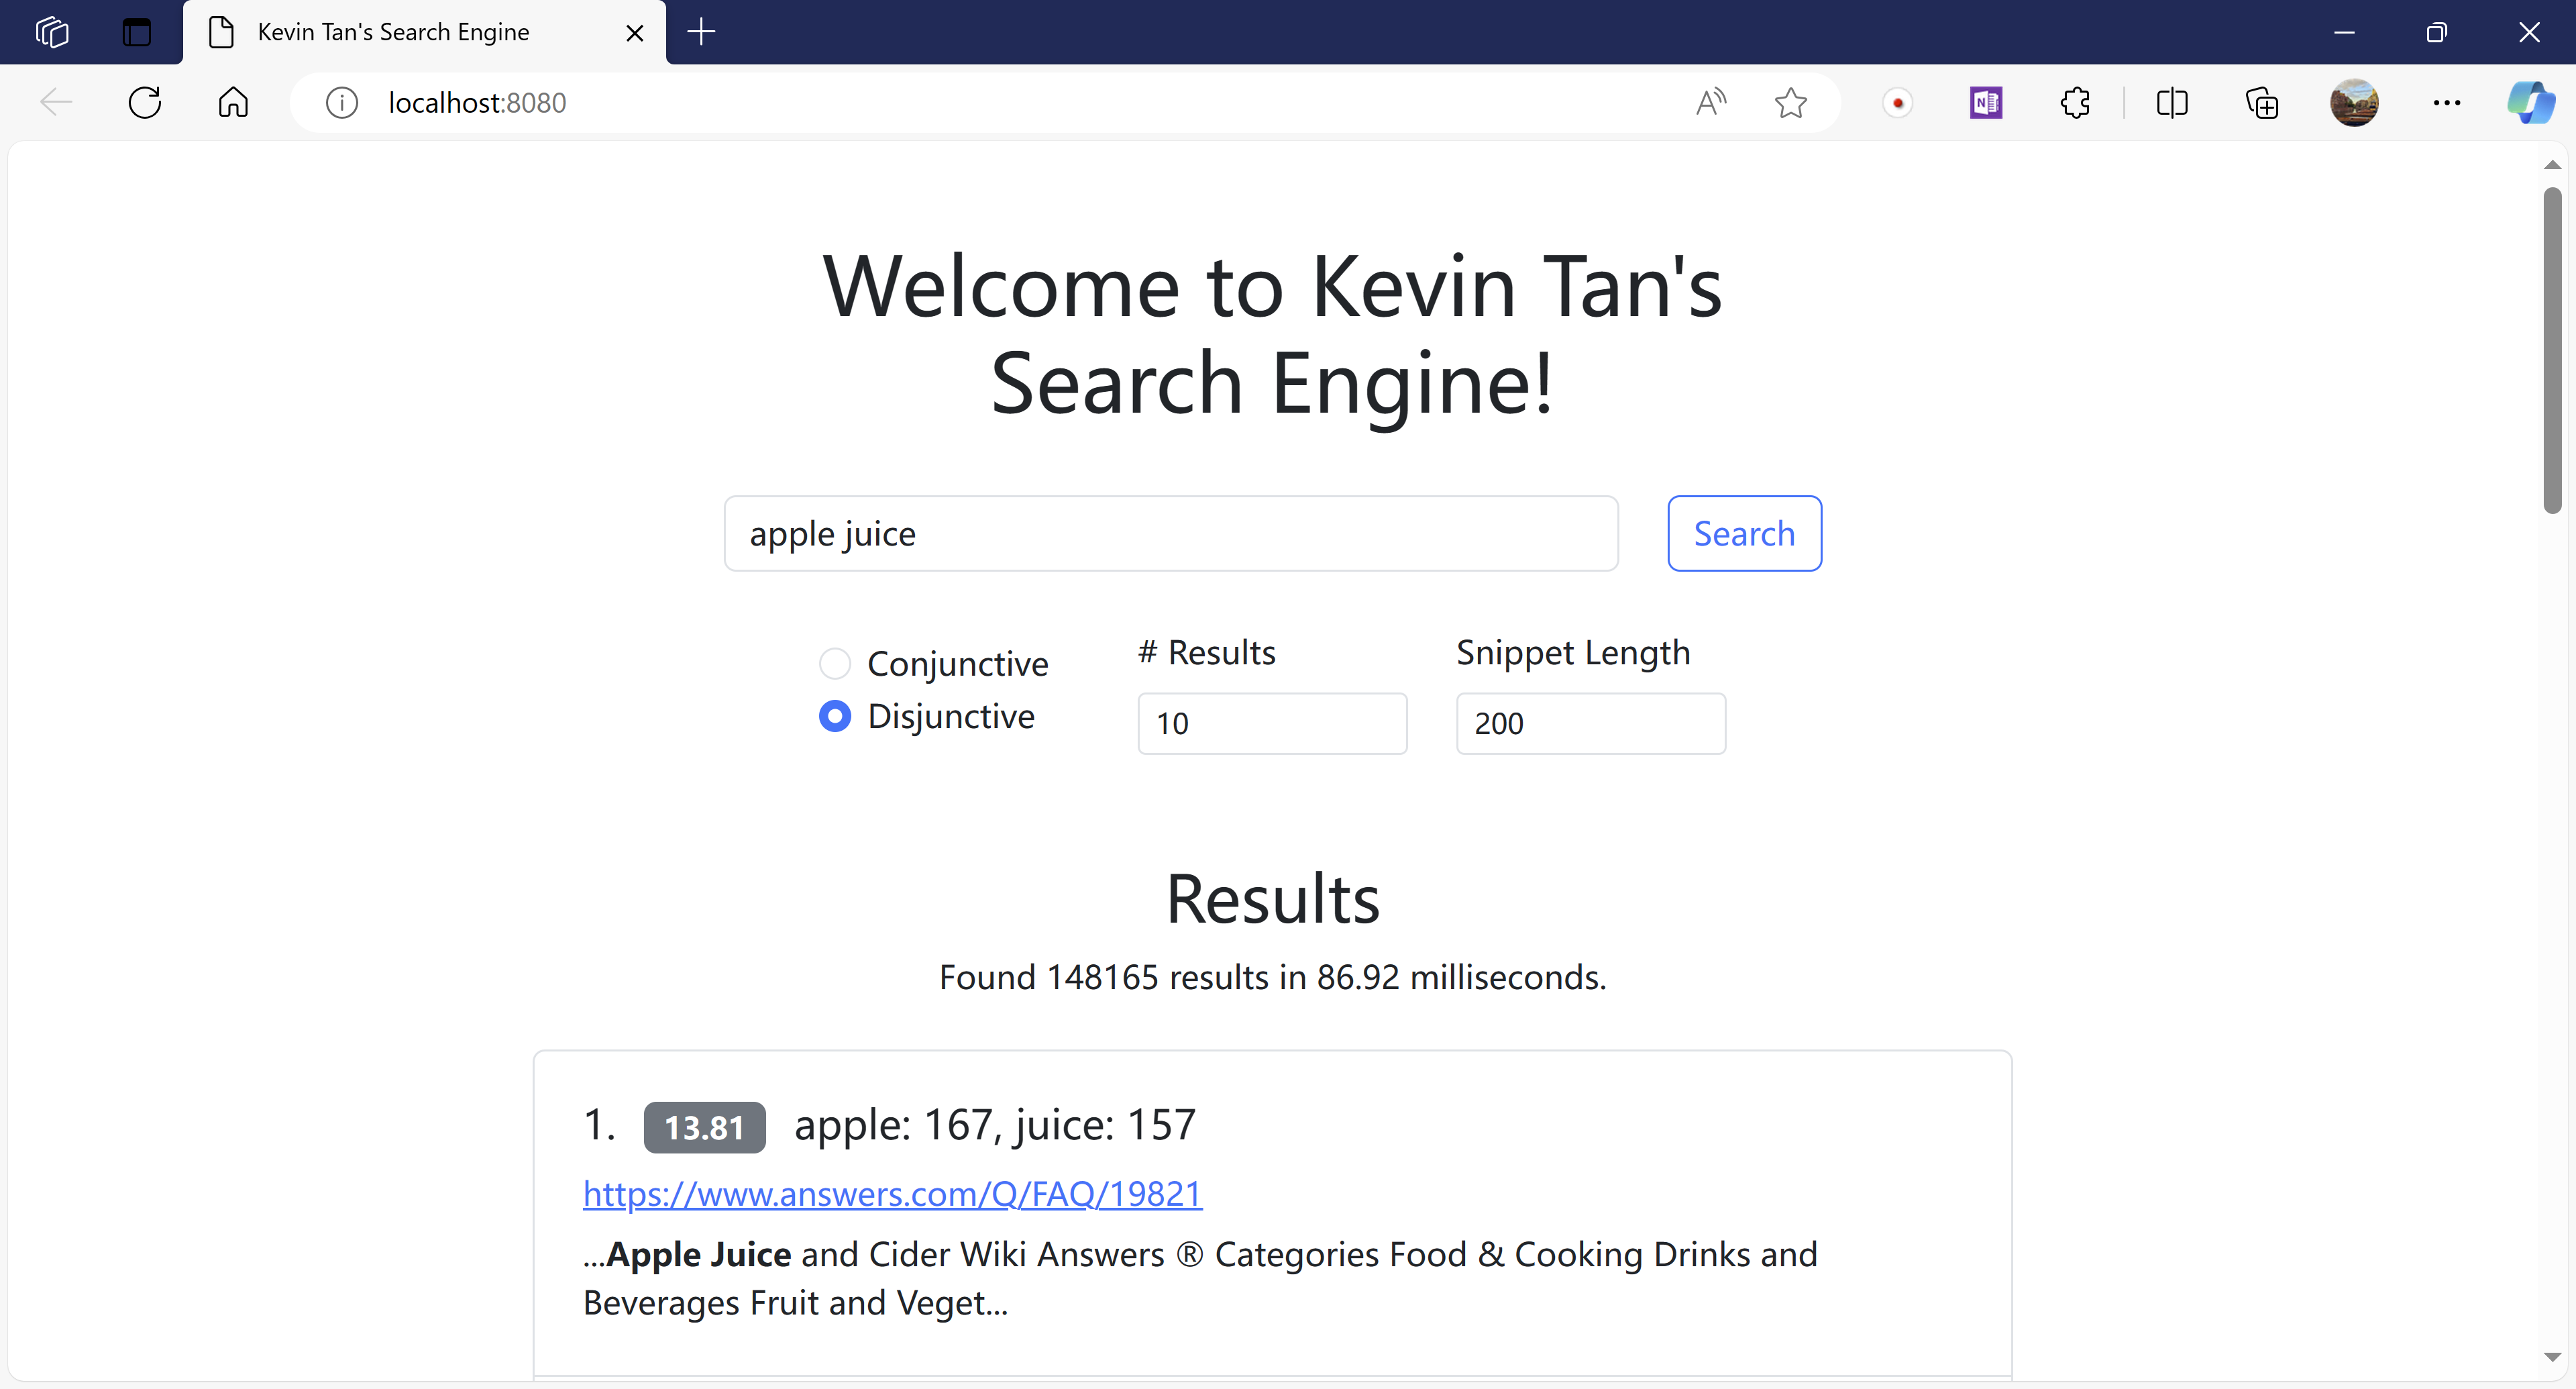
\includegraphics{readme.assets/image-20231112215247864.png}
  \vspace{-8pt}
  \caption{Conjunctive queries typically cost less time than disjunctive queries}
  \label{disjunctive}
\end{figure}

\hypertarget{v-conclusion-and-future-work}{%
\section{V. Conclusion and Future
Work}\label{v-conclusion-and-future-work}}

In this paper, a web search engine is built from scratch, supporting
indexing a large dataset into a compressed form with limited memory,
searching by multilingual conjunctive or disjunctive queries, and
interacting from a responsive web page or command lines. The program
achieves good efficiency and maintainability. In the future, more work
can be achieved, such as improving the ranking by PageRank or using
Large Language Models (LLMs) to generate better snippets. By designing
and implementing the search engine, the author gains a deeper
understanding of web search engines and acquires practical skills for
similar tasks.

\begin{thebibliography}{99}

\bibitem{c1}S. E. Robertson, S. Walker, S. Jones, M. Hancock-Beaulieu, and
M. Gatford. 1994. Okapi at TREC-3. In \emph{Proc. TREC}.

\bibitem{c2}A. Trotman, X-F. Jia, and M. Crane. 2012. Towards an efficient
and effective search engine. In \emph{Wkshp. Open Source IR}. 40--47.

\end{thebibliography}

\end{document}